
\section{Graphical representation}
\label{ariaid-title3}

The graphical representation of the Application Profile is provided in
the form of an UML class
diagram\footnote{Class diagram,
	\url{https://en.wikipedia.org/wiki/Class_diagram}} and is depicted
in the figure below. The boxes represent classes while the arrow
connections represent properties establishing relations to other
classes. The attributes inside boxes represent properties providing
either literal data values or relation to other classes that omitted
from the diagram. Both, arrows and attributes, are labelled with the
property names prefixed with the namespace where they are defined.

\begin{figure}[!ht]
	\centering
	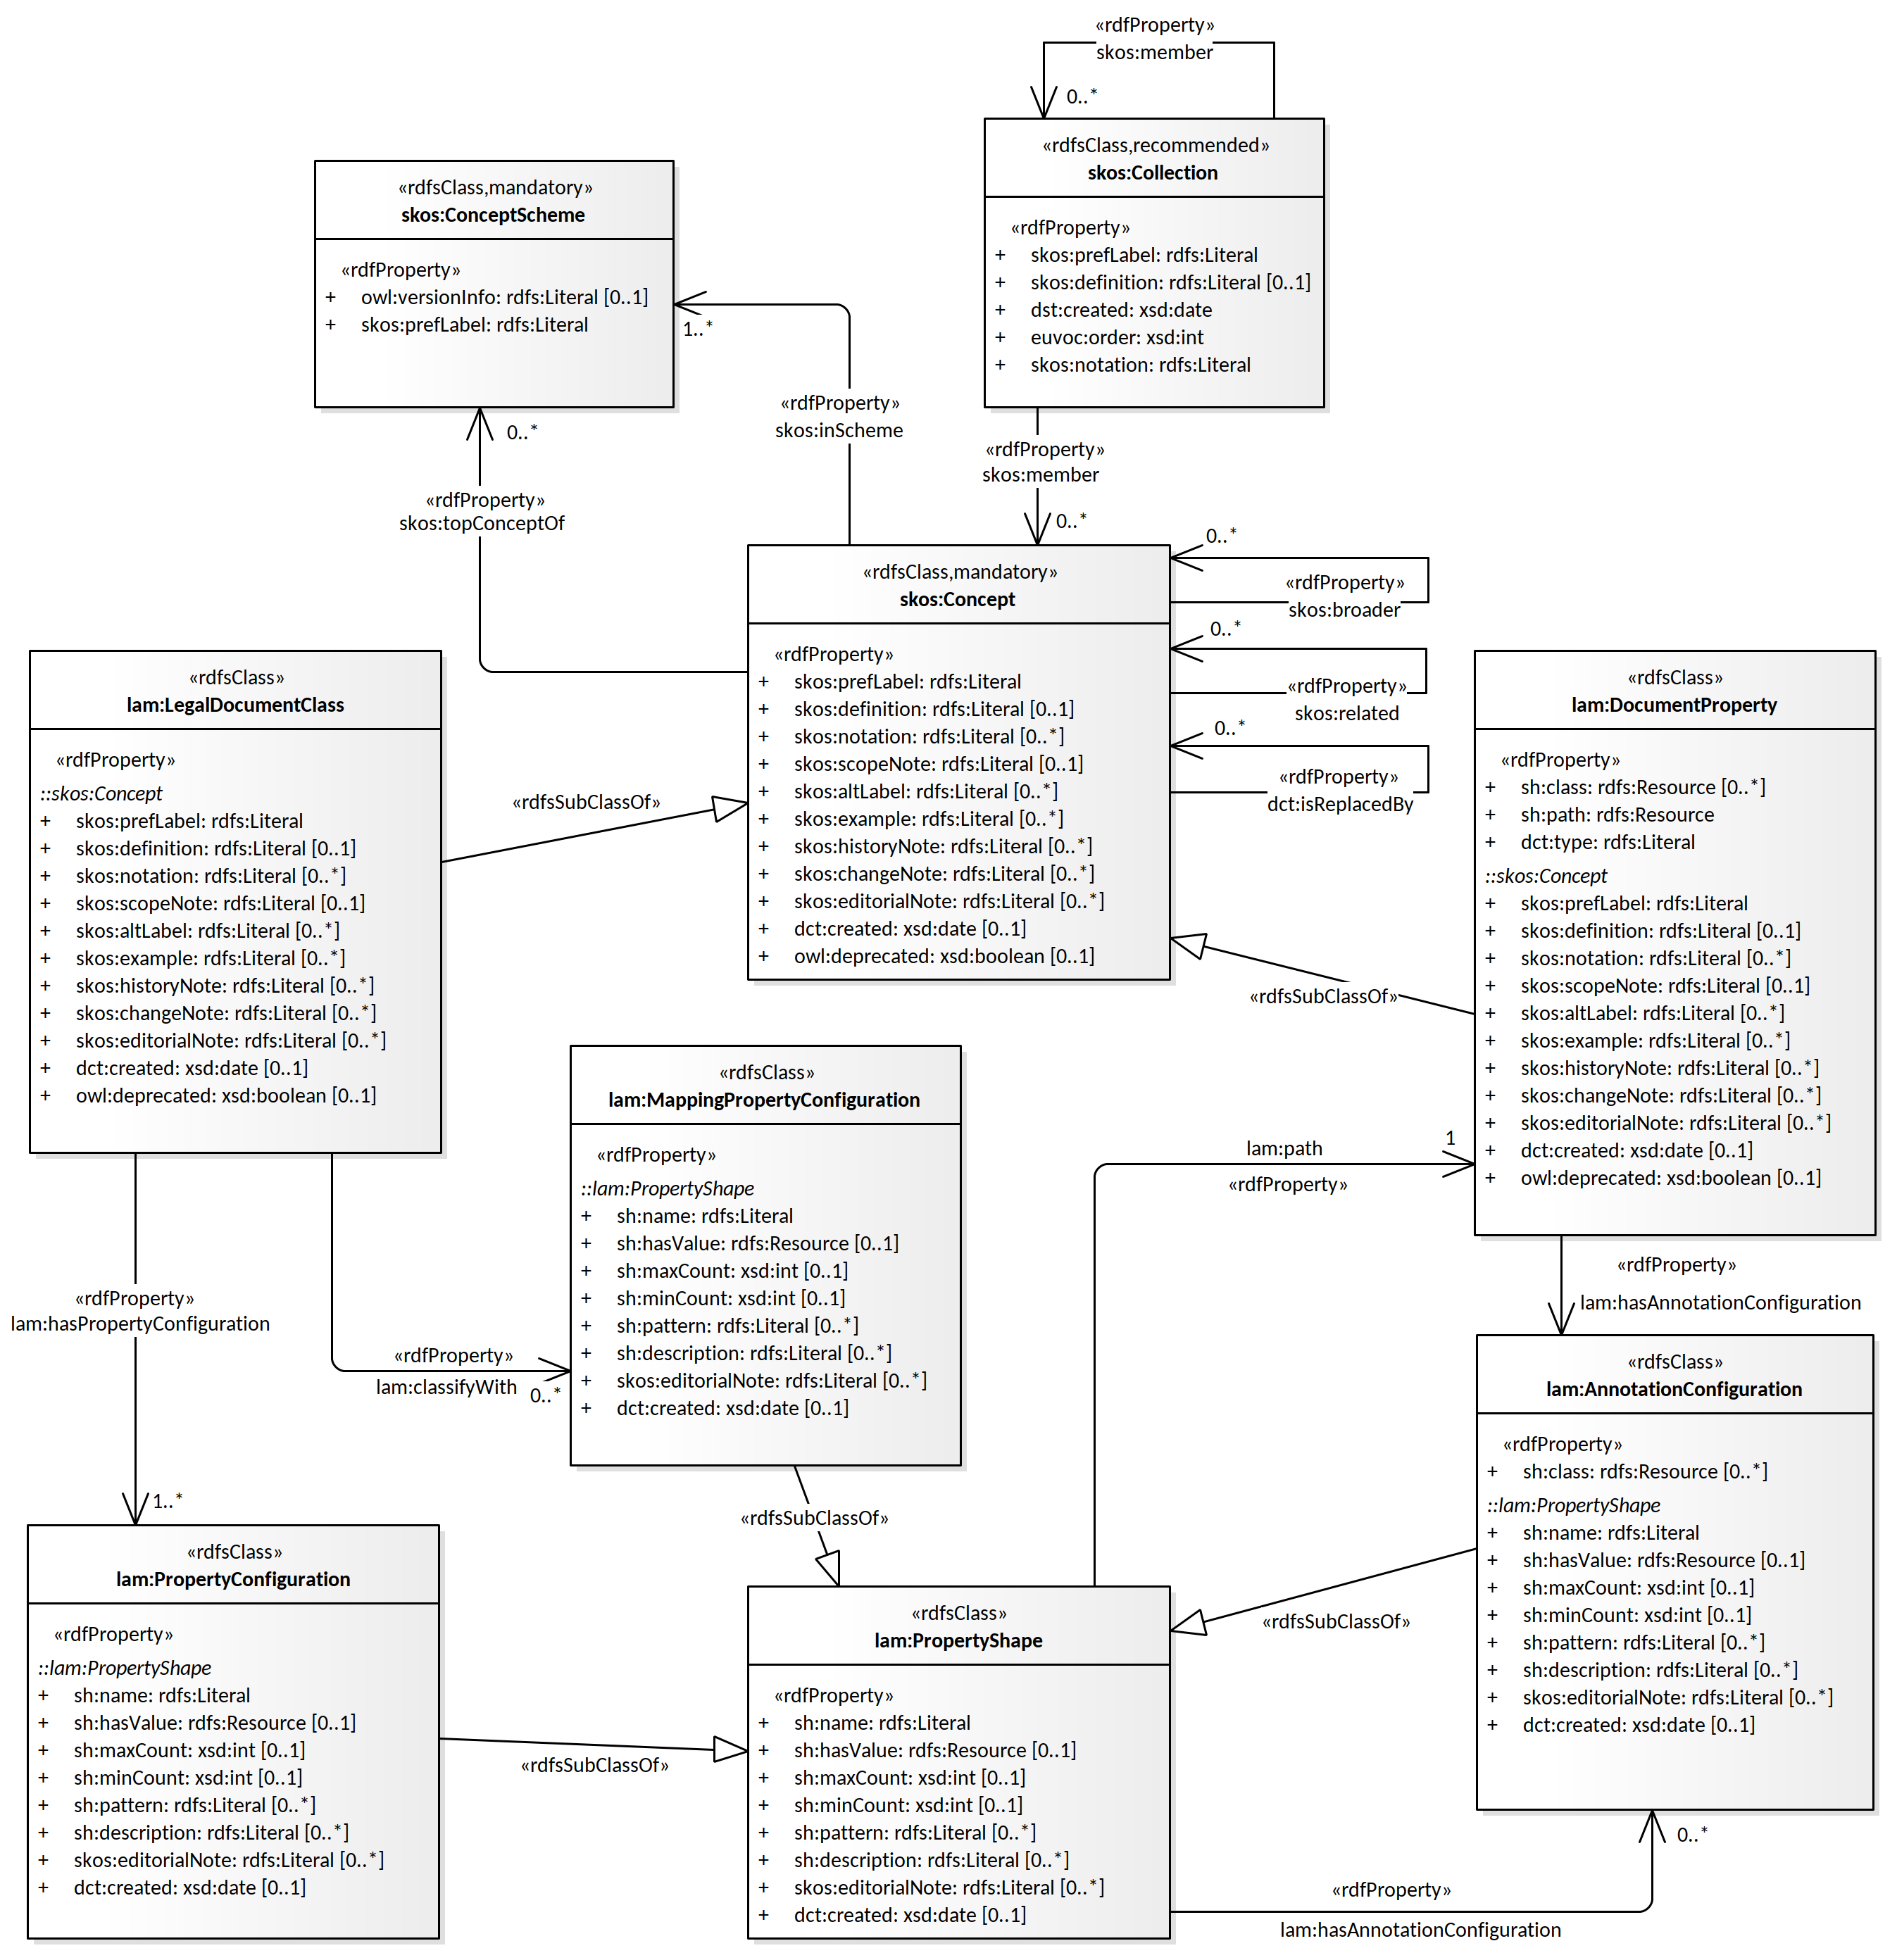
\includegraphics[width=0.95\textwidth]{images/lam-skos-ap-2021.png}
	\caption{UML class diagram for the SRC-AP-VB3 application profile}
\end{figure}

The cardinality specifications on the connector (\_ .. \_) arrows and
next to the attributes, marked in square brackets ( {[} {]} ) represent
constraints on how the property may be employed on the class instances
and has a normative meaning. The first number means minimum cardinality
constraint and the second means maximum cardinality constraint. The
minimum cardinality constraint is zero (0 .. \_ ) for optional
properties and one (1 .. \_) for mandatory properties. The maximum
cardinality constraint is usually unspecified ( \_ .. *) or limited to
one (\_ .. 1) and has no normative value in this application profile. If
the cardinality is not specified then the implied meaning is exactly one
(1..1).

The stereotypes, marked in the double angle brackets
(\textless{}\textless{} \textgreater{}\textgreater{}), used in the
diagram are based on RDFS model. They have an indicative and not a
semantic value. The "mandatory", "optional" and "recommended"
stereotypes are normative and have the meaning defined in the
\href{ap-terminology.html\#ap-terminology}{terminology section} .

In the curly brackets (\{ \}) are provided the constraints on the
property values. These constraints refer to controlled list of values
that should meet \href{ap-controlled-vocabulary-requirements.html}{a
minimum set of requirements}.


